\chapter{Überprüfung der Hypothese 5 \textit{\textcolor{gray}{(Autoren: Philipp und Patrick)}}}
\label{chap:hypothese5}


\section{Vorgehensweise}
Mit der Hypothese \gqq{Die Einführung einer 4-Tage-Woche führt zu einer 
Steigerung der Attraktivität des Arbeitgebers} wird - wie schon in \ref{tab:hyptothesen} beschrieben - der 
Fokus auf die Auswirkung der 4-Tage-Woche auf die Arbeitgebenden gelegt. 

\paragraph{Identifikation der relevanten Variablen}
In einem ersten Schritt werden die Variablen aus der durchgeführten Umfrage identifiziert, die für die 
Überprüfung der Hypothese relevant sein könnten.

Als erstes ist dort die Frage \gqq{Könnte die Implementierung einer 4-Tage-Arbeitswoche die Attraktivität 
Ihres Unternehmens / Ihrer Organisation steigern?} zu nennen. Diese dient für die folgende Analyse als abhängige 
Variable, da sie die wahrgenommene Attraktivität des Arbeitgebenden in der untersuchten Stichprobe abbildet.

Zu den unabhängigen Variablen zählen in diesem Fall die erhobenen Daten, welche es ermöglichen die Meinung 
einzelner Teilgruppen in mitten der Befragten gesondert zu betrachten. Daraus kann sich erkennen lassen, wie diese
Eigenschaften die wahrgenommene Attraktivität der Arbeitgebenden nach Einführung einer 4-Tage-Woche beeinflussen.
Die folgenden unabhängigen Variablen sind:

\begin{itemize}
  \item Alter
  \item Geschlecht
  \item Kinder (Ja/Nein)
  % \item (Beschäftigungsverhältnis)
  % \item Branche
  % \item Körperliche Beanspruchung
  \item Die Position im Unternehmen (Führungskraft oder nicht)
\end{itemize}

\paragraph{Ausgewählte Analyseverfahren} Begonnen wird mit der allgemeinen Betrachtung der Meinung 
aller Befragten um das generelle Stimmungsbild der Stichprobe zu ermitteln. Anschließend werden die Auswirkungen
der einzelnen Variablen, welche zuvor genannt worden sind, auf die wahrgenommene Attraktivität des Arbeitgebenden 
untersucht.

Für die allgemeine Betrachtung wird ein Histogramm der abhängigen Variable erstellt, um die Verteilung 
der Antworten zu visualisieren. Für eine weitere Betrachtung der Daten, werden 
dazu der Modalwert (Modus), Median und Mittelwert der Antworten berechnet.

In der weiteren Betrachtung wird die Auswirkung einzelner unabhängigen Variablen auf die Meinung zur 
Attraktivität des Arbeitgebenden untersucht. Hierfür werden Kreuztabellen erstellt, um erste
Zusammenhänge zu erkennen. 
Anschließend werden darauf aufbauend abhängig von der Beschaffenheit des Merkmals
weitere Analyseverfahren angewendet. 

\section{Analyse}

Die allgemeine Meinung der Befragten zur Attraktivität des Arbeitgebenden wird in dem folgenden Histogramm 
\ref{fig:attraktivitaet_verteilung} dargestellt. Dabei konnten die Befragten zwischen den folgenden Antwortmöglichkeiten wählen,
welchen mit den dabei stehenden Nummern codiert worden sind: \gqq{Ja(1)}, \gqq{Eher Ja (2)},
\gqq{Neutral (3)}, \gqq{Eher Nein (4)} und \gqq{Nein (5)}. 

% Die Verteilung der Antworten zeigt, dass die Mehrheit der
% Befragten die Einführung einer 4-Tage-Woche durch den Arbeitgebenden als attraktiv empfinden.

Das Histogramm zeigt eine klare Schieflage nach links, was widerspiegelt, dass die Verteilung 
asymmetrisch und die meisten Antworten im Bereich der höheren Attraktivität (1 - Ja und 2 - Eher Ja) liegen. 
Dies spiegelt sich auch im Mittelwert wieder, welcher mit 1,86 ebenfalls im Bereich der höheren Attraktivität
zu finden ist. Der Modalwert (Modus) liegt bei 1 (Ja), was bedeutet, dass die meisten Befragten die Einführung einer 
4-Tage-Woche als Attraktivitätssteigernd bei einen Arbeitgebenden empfinden. Der Median
liegt bei 2 (Eher Ja), was ebenfalls auf eine positive Meinung der Befragten zur Attraktivität des Arbeitgebenden
hinweist.


\begin{figure}[h][h]
    \centering
    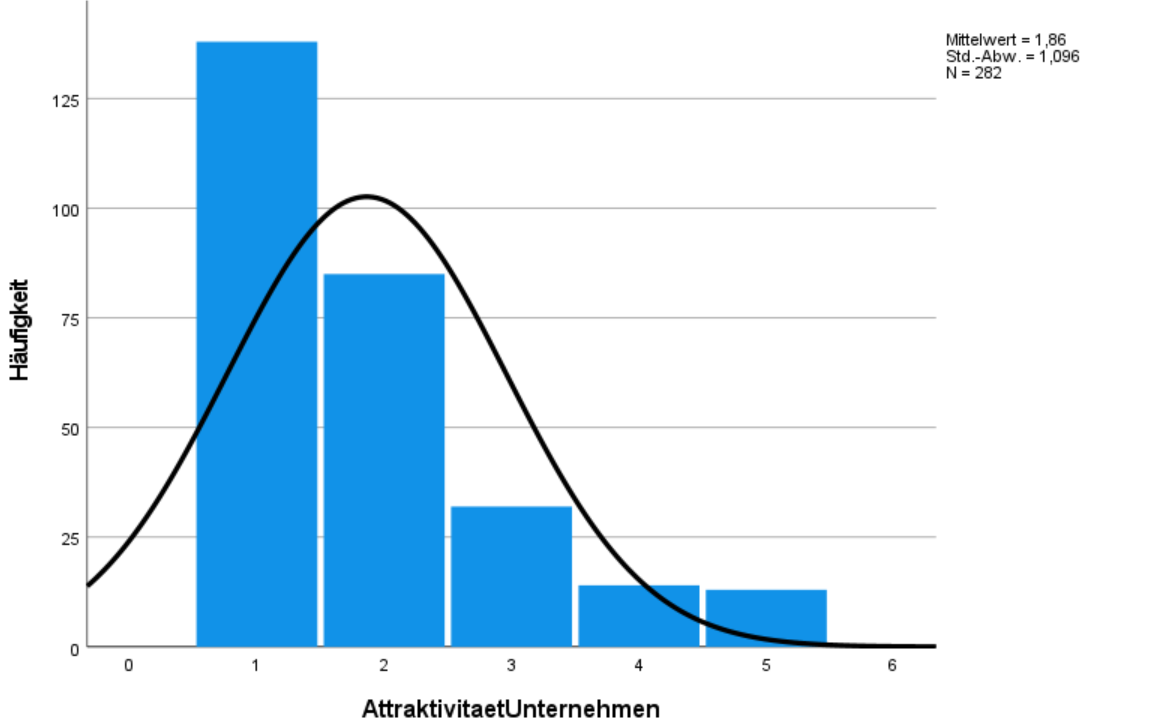
\includegraphics[width=0.7\textwidth]{04_Artefakte/01_Abbildungen/hypothese_5/attraktivitaet_histogram.png}
    \caption{Verteilung der Antworten zur Attraktivität des Arbeitgebenden}
    \label{fig:attraktivitaet_verteilung}
\end{figure}

\paragraph*{Alter}

% - Haben auch probiert, divers und keine Angabe raus zu nehmen um weniger Verzerrung zu haben und ordninale regression probiert. 
% Allergings war das pseudo R^2 sehr niedrig und die Signifikanz sehr hoch, was darauf hindeutet, dass das Modell nicht gut passt. 
% Daher haben wir uns für die Kreuztabelle entschieden mit ~0,01 sehr niedrig was darauf hinweise, dass das Modell nicht wirklich gut ist.

Die Verteilung der Antworten zur Attraktivität des Arbeitgebenden unter Berücksichtigung des Alters ist in Abbildung \ref{fig:attraktivitaet_alter}
zu finden. Es wurde sich hierbei für ein auf die Größe der Stichprobe normiertes Balkendiagramm entschieden, um die Verteilung der Antworten
relativ zur Anzahl der Befragten in den jeweiligen Altersgruppen darzustellen.

Ausgenommen der Altersgruppe 66+ geben die Befragten aller Altersgruppen überwiegend an, dass sie die Meinung vertreten die 
Attraktivität des Arbeitgebenden würde durch das Angebot einer 4-Tage-Woche steigen. Es fällt allerdings auf, dass mit 
zunehmendem Alter der Anteil der \gqq{Ja(1)} Stimmen abnimmt und der Anteil der \gqq{Eher Ja(2)} Stimmen zunimmt. Eine 
Korrelationsanalyse nach Spearman zeigt einen fast schon mittleren Zusammenhang zwischen dem 
Alter und der Meinung zur Attraktivität ebenfalls auf, mit einem Korrelationskoeffizienten von 0,216 auf einem Signifikanzniveau von 
0,01 (siehe Abbildung \ref{fig:korrelation_alter}).

\begin{figure}[h]
  \centering
  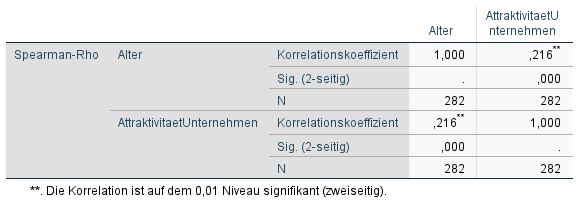
\includegraphics[width=0.7\textwidth]{04_Artefakte/01_Abbildungen/hypothese_5/korrelation_alter.png}
  \caption{Spearman Korrelationsanalyse zwischen Alter und Attraktivität des Arbeitgebenden}
  \label{fig:korrelation_alter}
\end{figure}

% Die Analyse zeigt, dass die Meinung zur Attraktivität des Arbeitgebenden nach Einführung einer 4-Tage-Woche sich nicht sonderlich zwischen den
% Altersgruppen unterscheidet. So geben Befragte aller Altersgruppen überwiegend an, dass sie die Meinung vertreten die Attraktivität des Arbeitgebenden würde sich
% so zumindest eher steigern. Lediglich in der Altersgruppe 66+ gibt es keine positiven Stimmen. Allerdings ist die Stichprobe in dieser Altersgruppe
% auch mit $n=2$ die kleinste und daher nicht repräsentativ für diese Gruppe.


\begin{figure}[h]
  \centering
  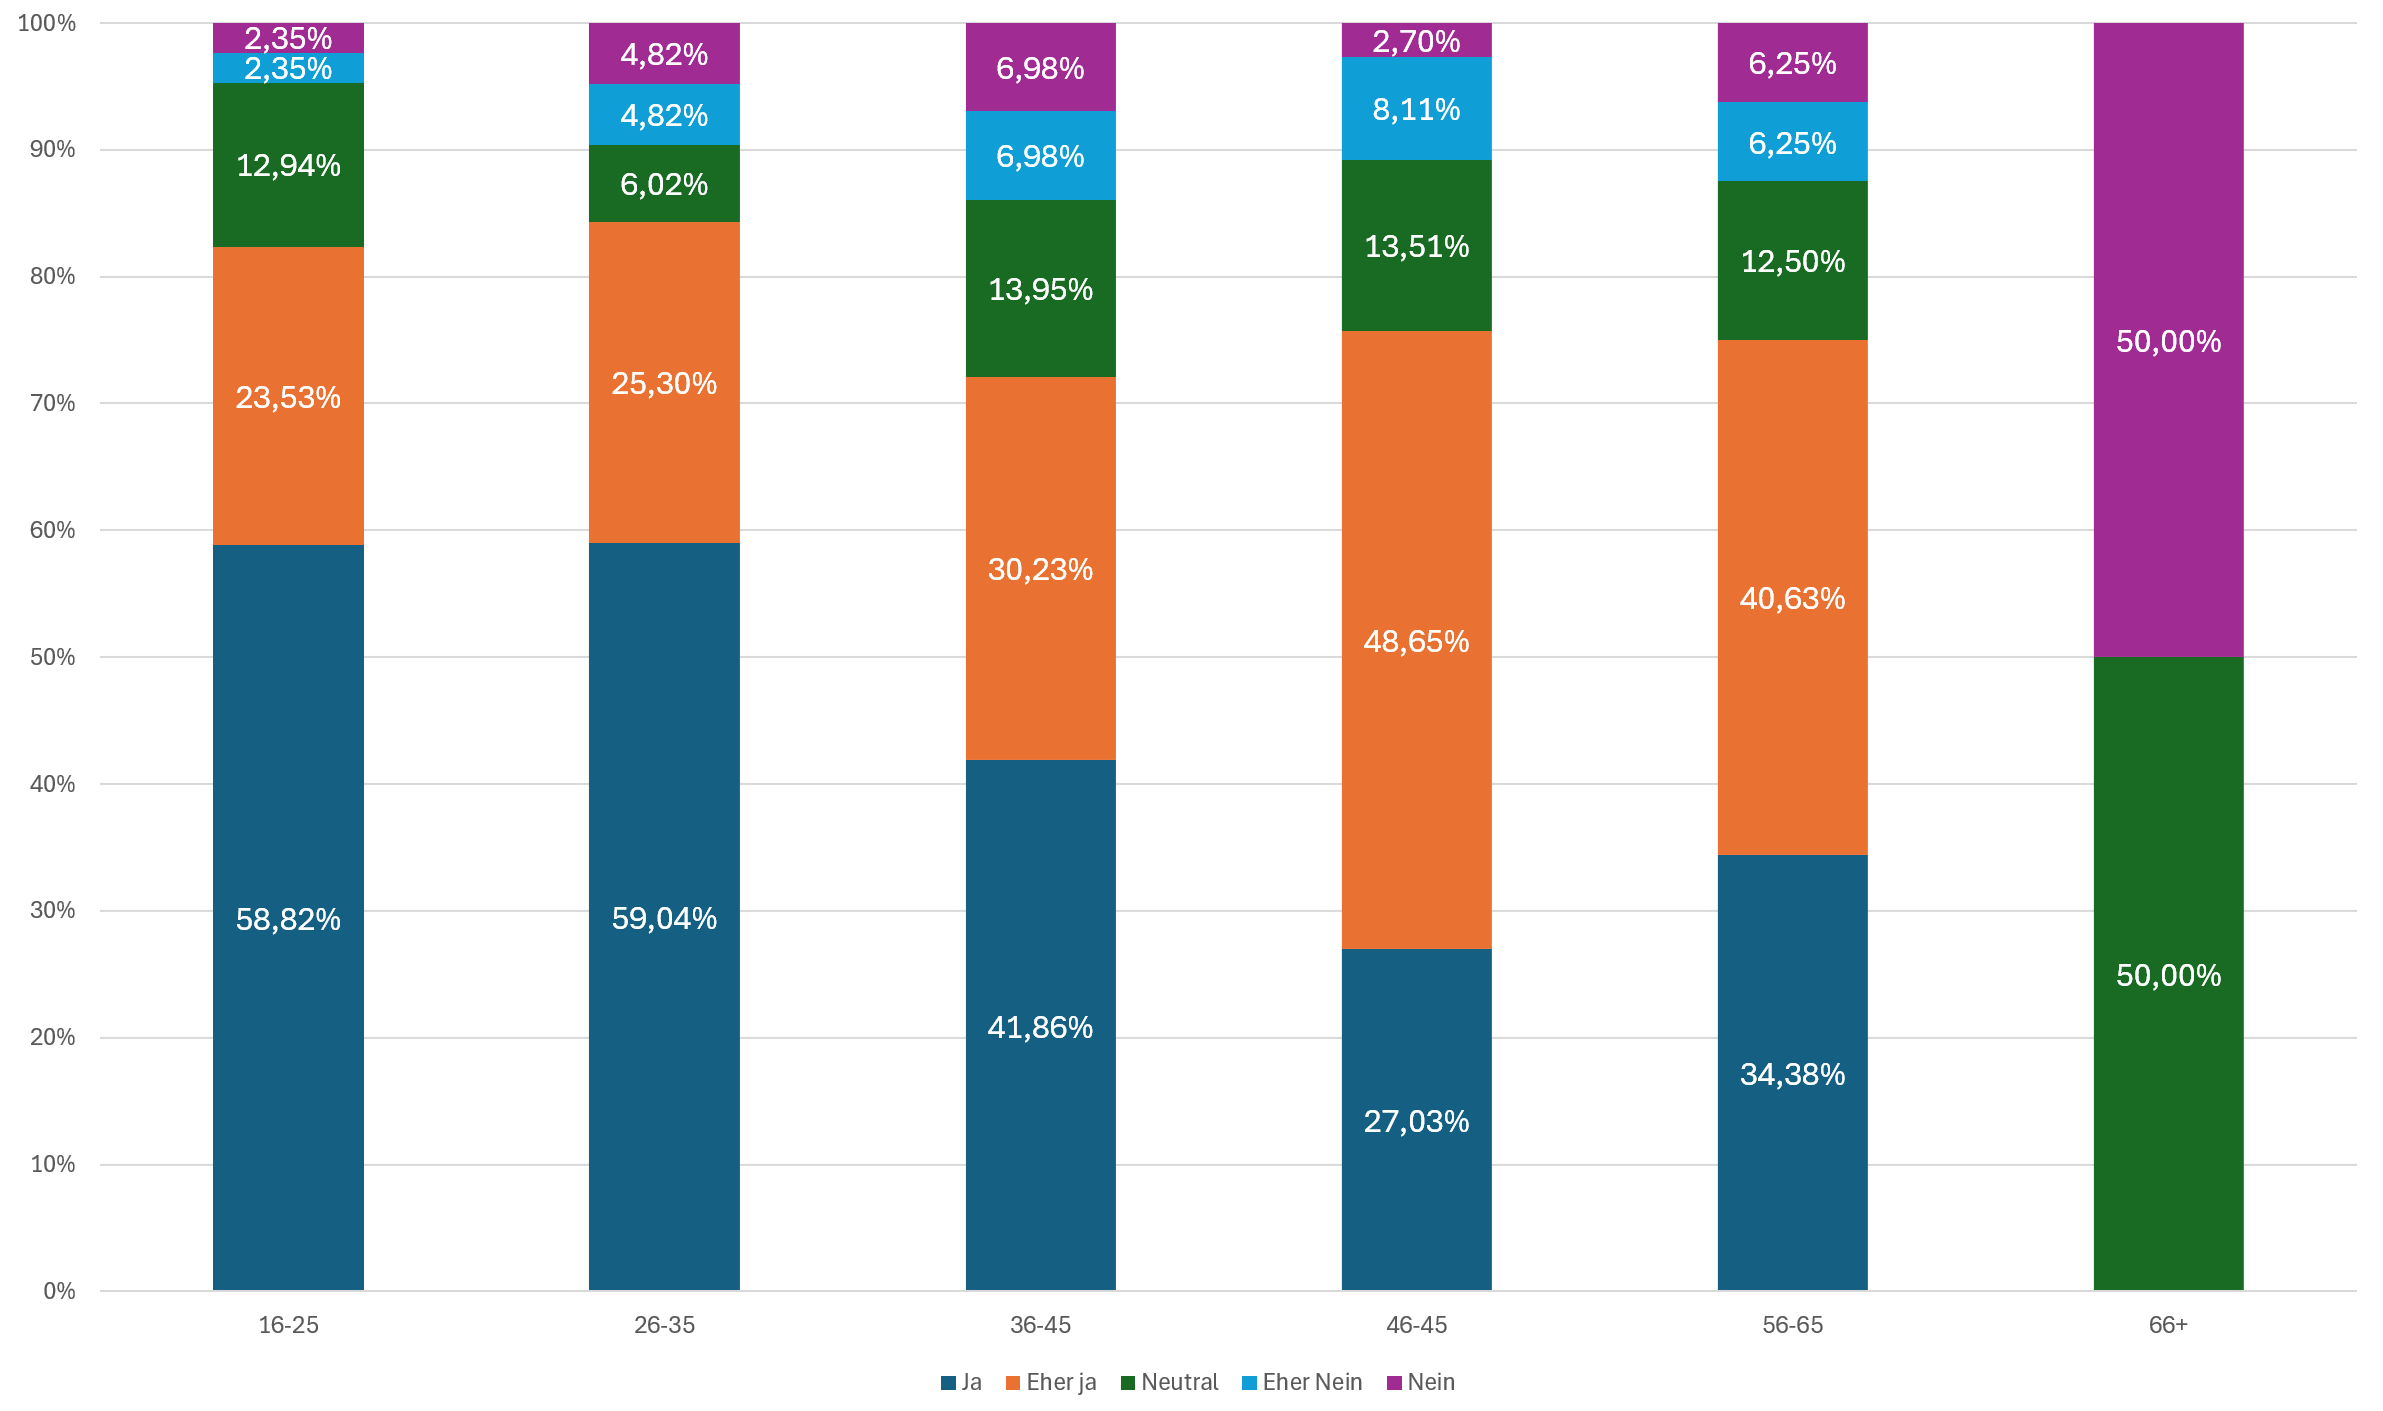
\includegraphics[width=0.7\textwidth]{04_Artefakte/01_Abbildungen/hypothese_5/attraktivitaet_alter.png}
  \caption{Verteilung der Antworten zur Attraktivität des Arbeitgebenden unter Berücksichtigung des Alters}
  \label{fig:attraktivitaet_alter}
\end{figure}

\paragraph*{Geschlecht}

Wie in Kreuztabelle \ref{tab:attraktivitaet_geschlecht} zu erkennen, variiert die Meinung zur Attraktivität des Arbeitgebenden
nach Einführung einer 4-Tage-Woche zwischen den Geschlechtern. So geben Frauen häufiger an, dass die
Attraktivität des Arbeitgebenden durch die Einführung einer 4-Tage-Woche steigen würde, als Männer. Dies zeigt sich
auch in der relativen Verteilung der Antworten. Ein kleiner Zusammenhang zwischen dem Geschlecht und der Meinung zur Attraktivität
kann auch durch die Korrelationsanalyse nach Spearman bestätigt werden, mit einem Korrelationskoeffizienten von 0,13 auf einem 
Signifikanzniveau von 0,05 (siehe Abbildung \ref{fig:korrelation_geschlecht}). Hier wurden die Antworten zu divers und keine Angabe 
zum Geschlecht aufgrund der geringen Anzahl an Antworten aus der Korrelationsanalyse ausgeschlossen.

\begin{table}[h]
  \centering
  \begin{tabular}{cl|r|r|r|r|r|r|r|r|r}
  & & \multicolumn{8}{c|}{Geschlecht} \\
  & & \multicolumn{2}{c|}{Weiblich} & \multicolumn{2}{c|}{Männlich} & \multicolumn{2}{c|}{Divers} & \multicolumn{2}{c|}{Keine Angabe} \\ \hline
  & Ja        & 73 & 54,89\% & 61 & 42,07\% & 3 & 100\% & 1 & 100\% \\
  & Eher Ja   & 36 & 27,07\% & 49 & 33,79\% & 0 & 0\%   & 0 & 0\%   \\
  & Neutral   & 15 & 11,28\% & 17 & 11,72\% & 0 & 0\%   & 0 & 0\%   \\
  & Eher Nein & 7  & 5,26\%  & 7  & 4,83\%  & 0 & 0\%   & 0 & 0\%   \\
  \multirow{-5}{*}{\rotatebox[origin=c]{90}{Attraktivität}} & Nein & 2 & 1,50\% & 11 & 7,58\% & 0 & 0\% & 0 & 0\%  \\ \hline
  &           & 133 & & 145 & & 3 & & 1 & & 282
  \end{tabular}
  \caption{Kreuztabelle der Attraktivität des Arbeitgebenden unter Berücksichtigung des Geschlechtes}
  \label{tab:attraktivitaet_geschlecht}
\end{table}

\begin{figure}[h]
  \centering
  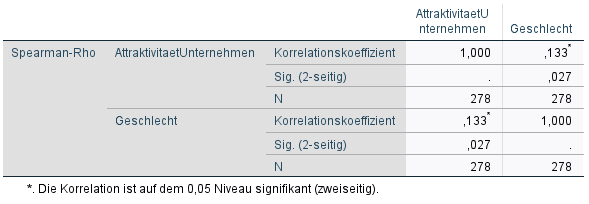
\includegraphics[width=0.7\textwidth]{04_Artefakte/01_Abbildungen/hypothese_5/korrelation_geschlecht.png}
  \caption{Spearman Korrelationsanalyse zwischen Alter und Attraktivität des Arbeitgebenden}
  \label{fig:korrelation_geschlecht}
\end{figure}


\paragraph*{Kinder}

Die Motivation für die Betrachtung des Zusammenhangs zwischen der Attraktivität des Arbeitgebenden und ob die befragte 
Person Kinder hat, beruht auf der Vermutung, dass die Person in diesem Fall mehr Wert darauf legt Zeit mit den Kindern verbringen
zu können. Die Kreuztabelle \ref{tab:attraktivitaet_kinder} zeigt allerdings auf, dass genau das Gegenteil der Fall zu sein scheint.
Die Teilnehmenden, die Kinder haben, geben häufiger an, dass die Einführung einer 4-Tage-Woche die Attraktivität 
des Arbeitgebenden nicht oder eher nicht steigen würde. Die Korrelationsanalyse zeigt zudem einen Zusammenhang auf mit
einem Korrelationskoeffizienten von -0,205 und signifikant auf dem 0,01 Niveau (siehe Abbildung \ref{fig:korrelation_kinder}).

\begin{table}[h]
  \centering
  \begin{tabular}{cl|r|r|r|r|r}
  & & \multicolumn{4}{c|}{Kinder} & \\
  & & \multicolumn{2}{c}{Ja} & \multicolumn{2}{c|}{Nein} & \\ \hline
  & Ja        & 35 & 33,65\%  & 103 & 57,87\%  & \\
  & Eher Ja   & 43 & 41,35\%  & 42  & 23,6\%  &  \\
  & Neutral   & 13  & 12,5\%  & 19  & 10,67\%  &  \\
  & Eher Nein & 8  & 7,69\%  & 6   & 3,37\%   &  \\
  \multirow{-5}{*}{\rotatebox[origin=c]{90}{Attraktivität}} & Nein & 5 & 4,8\% & 8 & 4,49\% &  \\ \hline
  &           & 104 &       & 178 &       & 282
  \end{tabular}
  \caption{Kreuztabelle der Attraktivität des Arbeitgebenden unter Berücksichtigung ob die befragte Person Kinder hat}
  \label{tab:attraktivitaet_kinder}
\end{table}

\begin{figure}[h]
  \centering
  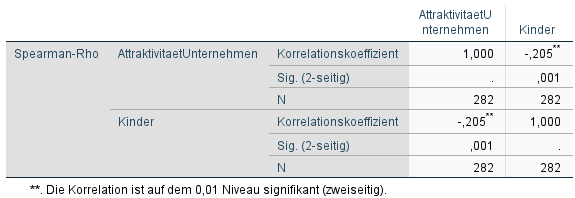
\includegraphics[width=0.7\textwidth]{04_Artefakte/01_Abbildungen/hypothese_5/korrelation_kinder.png}
  \caption{Spearman Korrelationsanalyse zwischen Kinder und Attraktivität des Arbeitgebenden}
  \label{fig:korrelation_kinder}
\end{figure}

\paragraph*{Führungskraft}

Wie auch in den vorangegangenen Absätzen wurde auch hier erst einmal eine Kreuztabelle erstellt, die in Tabelle \ref{tab:attraktivitaet_fuehrungskraft}
zu finden ist.
Wie sich aus der Tabelle ablesen lässt, geben Führungskräfte im Vergleich zu nicht Führungskräften häufiger an, dass die Einführung
einer 4-Tage-Woche die Attraktivität des Arbeitgebenden nicht oder eher nicht steigern würde. Dies zeigt sich auch in der relativen 
Verteilung der Antworten. Die Korrelationsanalyse zeigt ebenfalls einen Zusammenhang auf mit einem Korrelationskoeffizienten von -0,205 
und signifikant auf dem 0,01 Niveau (siehe Abbildung \ref{fig:korrelation_fuehrungskraft}).


\begin{table}[h]
  \centering
  \begin{tabular}{cl|r|r|r|r|r}
  & & \multicolumn{4}{c|}{Führungskraft} & \\
  & & \multicolumn{2}{c}{Ja} & \multicolumn{2}{c|}{Nein} & \\ \hline
  & Ja        & 25 & 36\%  & 113 & 53\%  & \\
  & Eher Ja   & 20 & 29\%  & 65  & 31\%  &  \\
  & Neutral   & 7  & 10\%  & 25  & 12\%  &  \\
  & Eher Nein & 7  & 10\%  & 7   & 3\%   &  \\
  \multirow{-5}{*}{\rotatebox[origin=c]{90}{Attraktivität}} & Nein & 10 & 14\% & 3 & 1\% &  \\ \hline
  &           & 69 &       & 213 &       & 282
  \end{tabular}
  \caption{Kreuztabelle der Attraktivität des Arbeitgebenden unter Berücksichtigung der Position als Führungskraft}
  \label{tab:attraktivitaet_fuehrungskraft}
\end{table}

\begin{figure}[h]
  \centering
  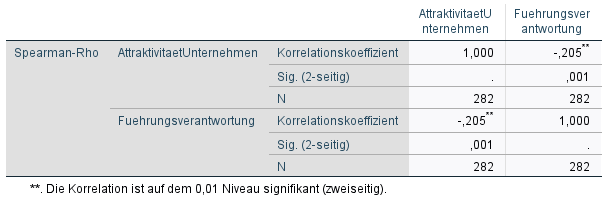
\includegraphics[width=0.7\textwidth]{04_Artefakte/01_Abbildungen/hypothese_5/korrelation_fuehrungskraft.png}
  \caption{Spearman Korrelationsanalyse zwischen Führungsverantwortung und Attraktivität des Arbeitgebenden}
  \label{fig:korrelation_fuehrungskraft}
\end{figure}

\section{Ergebnis}

Die Untersuchung des Zusammenhangs zwischen den unabhängigen und der abhängigen Variable gestaltete sich in der Analyse etwas schwieriger als vorhergesehen, 
da hier die unabhängigen Variablen nominal - und in den letzten beiden Fällen sogar dichotom - sind, die abhängige Variable jedoch ordinal.

Davon abgesehen zeigen die Analysen in diesem Kapitel, dass die Meinung zur Attraktivität des Arbeitgebenden besonders im 
Zusammenhang mit drei Variablen zu stehen scheint: dem Alter (vgl. Abbildung \ref{fig:attraktivitaet_alter}), 
ob die befragte Person Kinder hat (vgl. Tabelle \ref{tab:attraktivitaet_kinder}) und ob die befragte Person eine Führungskraft ist 
oder nicht (vgl. Tabelle \ref{tab:attraktivitaet_fuehrungskraft}). Alle weisen einen Korrelationskoeffizienten von über 0,2 auf. 

Dabei scheint es so, dass Befragte ohne Kinder dem Arbeitgebenden unter 
einer 4-Tage-Woche eine höhere Attraktivität zuschreiben als Befragte mit Kindern, was dem Gegenteil der ursprünglichen Vermutung entsprach. 

% Ähnlich verhält es sich bei Führungskräften, die dem Arbeitgebenden
% unter einer 4-Tage-Woche ebenfalls eine geringere Attraktivität zuschreiben als nicht Führungskräfte. 
% Frauen hingegen scheinen dem Arbeitgebenden
% unter einer 4-Tage-Woche im Allgemeinen eine höhere Attraktivität zuzuschreiben als Männer.

% Die Forschenden hatten zu Beginn zwar auch einen Zusammenhang mit dem Geschlecht der Befragten erwartet, jedoch konnte dies anhand
% der Stichprobe nicht bestätigt werden da sich die Meinung zur Attraktivität des Arbeitgebenden nicht signifikant zwischen den 
% Altersgruppen unterschied.

Abseits der genauer betrachteten Variablen scheint die Branche der Befragten zwar einen Einfluss auf die Meinung zur Attraktivität des Arbeitgebenden unter einer 4-Tage-Woche
zu haben, allerdings war die Stichprobe in diesem Fall zu klein, um belastbare Aussagen treffen zu können.

Abschließend lässt sich sagen, dass die Hypothese 5, dass die Einführung einer 4-Tage-Woche zu einer Steigerung der Attraktivität des Arbeitgebenden führt,
nicht vollständig bestätigt werden kann. Vielmehr scheint die Meinung zur Attraktivität des Arbeitgebenden unter einer 4-Tage-Woche von weiteren Faktoren
wie dem Alter, ob die befragte Person Kinder hat und ob die befragte Person eine Führungskraft ist oder nicht, abzuhängen.
Es lässt sich aber eine Tendenz erkennen, dass die Mehrheit der Befragten einen Arbeitgebenden, der eine 4-Tage-Woche einführt, als attraktiver empfinden.